%==========================================================================
%Template File for Monthly Lectual Meeting
%2006/05/22 (kkobayashi@mikilab.doshisha.ac.jp)
%==========================================================================
\documentclass[a4paper,9pt,twocolumn]{jsarticle}
\usepackage{mlm2.0}
\usepackage{epsf}
\pagestyle{plain}
\usepackage{url}
\usepackage{subfigure}
\setcounter{page}{1}
\usepackage{geometry}
\geometry{left=25mm,right=25mm,top=20mm,bottom=30mm}
%\usepackage[dvips]{graphicx}

\begin{document}
\twocolumn[
%---------------------------------------------------------------------------        % ヘッダ    書式:\beginheader{回}{年}{月}
%---------------------------------------------------------------------------
\beginheader{170}{2016}{04}
%---------------------------------------------------------------------------
% 発表題目    書式:\title{日本語}{英語} 「\\」で改行できます
%---------------------------------------------------------------------------
\title%
{git}%
%{更なる大容量化を目指して 進化しつづける次世代光メディア}

%---------------------------------------------------------------------------
% 著者名      書式:\author{日本語著者名}{英語著者名}
%---------------------------------------------------------------------------
\author{山下 俊樹,外村 篤紀\\Toshiki YAMASHITA,Atsuki TONOMURA}

%---------------------------------------------------------------------------
\endheader
%\begin{abstract}
%---------------------------------------------------------------------------
%Recently, a DVD attracts attention along with the image and the digitization of the sound. The standards of these DVD are complicated. So, in this paper, the standards of the DVD are summarized and the DVD of the next generation is refered. 
%---------------------------------------------------------------------------
%\end{abstract}
]

%---------------------------------------------------------------------------
% 本文
%---------------------------------------------------------------------------

\section{はじめに}
近年,コンピュータープログラムは大規模化し,その更新頻度は増加の一途を辿っている.そこで,コンピューター上で作成,及び編集されるファイルの変更履歴を管理するためのバージョン管理システムが注目を集めている.現在では,かつて主流であったSVNに代わり,より高機能なgitへの移行が進んでいる.本報告では,gitの概要と関連サービスについて述べる.

\section{gitとは}
git(ギット)とは,分散型バージョン管理システムの1つであり,従来用いられてきた集中型バージョン管理システムに変わり登場した.その概要を以下の\fgref{git}に示す.

\begin{figure}[h]
\centering
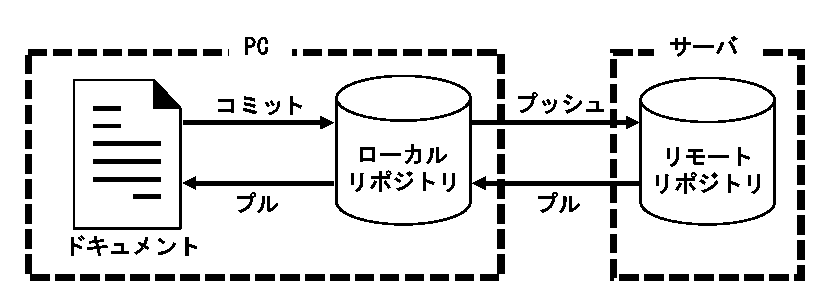
\includegraphics[width=70mm]{img/git.eps}
\caption{gitの概要}
\label{git}
\end{figure}

gitで管理されるファイルやディレクトリは,リポジトリと呼ばれる一種のデータベースにその変更が蓄積される.分散型バージョン管理システムにおけるリポジトリには,サーバー上に配置され,複数ユーザーで利用するリモートリポジトリと,個人のPC内に配置され,その個人が利用するローカルリポジトリの二種類がある.ユーザーがファイル等の変更をローカルリポジトリに記録する作業をコミットと呼び,これを実行すると前回のコミットからの差分が記録される.以前のコミットの時点の状態に戻す操作,及び後述するブランチを切り替える操作をチェックアウトと呼ぶ.また,ローカルリポジトリの変更をリモートリポジトリにアップロードする作業をプッシュ,リモートリポジトリからローカルリポジトリに変更をダウンロードする作業をプルと呼ぶ.コミットやプッシュを行うことで作業成果を記録し,プルを行うことで他者の作業成果を統合することができる.

次に,gitの機能の一つであるブランチについて述べる.その一例を以下の\fgref{branch}に示す.

\begin{figure}[h]
\centering
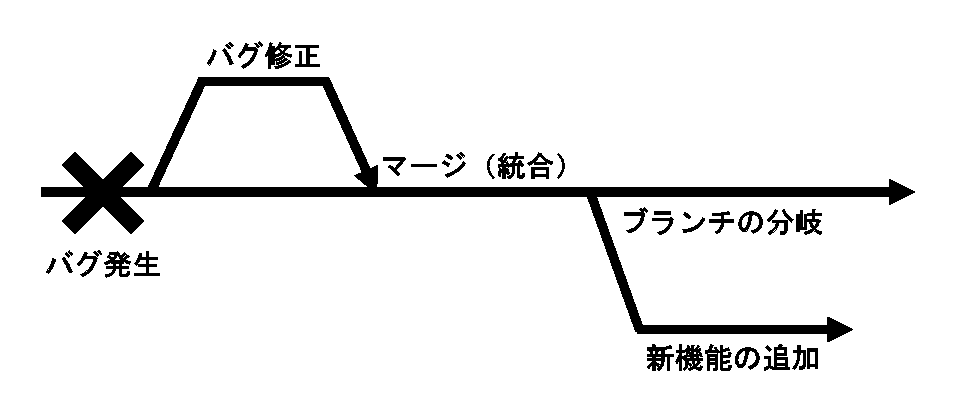
\includegraphics[width=80mm]{img/branch.eps}
\caption{ブランチの一例}
\label{branch}
\end{figure}

ブランチとは,変更履歴の流れを分岐する作業と分岐後の流れを指す.また,ブランチ同士の結合をマージと呼ぶ.ブランチ同士は独立しており,他のブランチの影響を受けない.また,\fgref{branch}のように,既に運用されているソフトウエアの開発を行っているブランチをmasterブランチとし,そのソフトウエアのバグを修正するために用意したブランチをbugfixブランチとする.この場合二つのブランチは独立しているため,ソフトウエアの運用を止めることなくバグの修正を行うことができるという利点を生む.

また,他のバージョン管理ソフトウエアに対するgitの利点は次の通りである.

\begin{itemize}
\item ローカルリポジトリを持つ
\item ブランチ機能が強力
\item 高速である
\end{itemize}

ローカルリポジトリによって,ネットワークに接続されていない環境でもコミットを行うことができる.あるいは,バグの修正のために個人のローカルリポジトリにコミットを適量蓄積し,修正が完了した後にリモートリポジトリにプッシュし他者に公開する等の使用方法が可能である.ブランチについては,マージを行う際に自動化されている比率が高いこと,マージが高速である等が挙げられる.更に,プログラム全体の動作が他サービスに比べて高速である.これは,gitがLinuxカーネル開発に使用するために開発されたため,OSカーネルのような巨大なソースコードの集合を高速に処理する必要があった経緯がある.

一方,欠点として,gitで扱えるファイルの種類はテキストベースのファイルに限られることが挙げられる.このため,書類作成のデファクト・スタンダードである,Microsoft Officeで作成したファイルを改変なしでは管理できない等の不具合を生じる.

\section{GitHubとは}
GitHubとは,gitを利用したSNSである.ユーザーはリモートリポジトリを無料で持つことができ,他のユーザーと協力してソースコードを管理できるサービスとして広まった.他のユーザーと協力するための機能として,コードレビュー,及びコメント機能等がある.コードレビューとは,ソースコードに含まれる誤りを検出,修正することを目的として行われるソースコードの査読を指す.これらの機能を用いることで,ユーザーのソースコードが他者の目に触れ,それに対してのコメントが付与される.その結果,ユーザーによる修正が行われ,ソースコードのバグが減少する,及び可読性が向上する等の利点を生む.

次に,フォーク機能について述べる.GitHubにおけるフォークはブランチの分岐操作を指す.この機能によって,ユーザーが他のユーザーのリポジトリからフォークしたブランチを用いて開発を行うことができる.利点としては,あるソフトウエアのデバッグを開発者以外のユーザーが行う事ができる,初心者がある程度完成されたソフトウエアをフォークすれば,フォーク元の本体には影響を与えず,様々な改変を行いながら学習ができる等が挙げられる.

更に,チケット機能についてである.GitHub内ではIssueと呼ばれているが,ここではチケットと同義として説明を行う.チケットとは,任意の作業をタスクに分割し,タスク一つ一つに対して割り振られるものである.開発者は発行されたチケットを取り,それに記されたタスク(バグ修正など)をこなし,タスクが完了するとコミットを行い,チケットを消去(クローズ)する.このようにタスクをチケットで管理することにより,作業の全容が把握しやすい,チームでの開発においてタスクの分配が行い易くなる等の利点がある.また,チケットを用いて行うチケット駆動開発は,アジャイル開発とも親和性が高いため,注目を集めている.

GitHubの利点は上記の通りである.一方,欠点としてGitHubで作成したリモートリポジトリは全て公開されるため,ソースコードを公開しない場合の多いWebデザイン等のソースコード管理には不具合が発生する.また,GitHubは外部サービスであるため,サーバー障害の様な事態が発生した場合に関連サービスが使用不可能になる危険性がある.実際に,2016年1月28日にサービス障害が発生し,多くのユーザーや企業が被害を被った\cite{news}.

GitHubに競合するサービスとして,BitBucketが挙げられる. Githubに対して,非公開のリモートリポジトリを作成できる,及びgit以外の分散型バージョン管理システムであるMercurialを使用できる等の利点がある.どちらのサービスもソーシャルコーディングの普及に貢献していると言えるが,現時点でのユーザー数はGitHubが圧倒的に多い.また,GitHubは対応する周辺サービスが多いこともあり,更にユーザーを増やしている.他にも競合するサービスがあるが,現段階ではGithubが最も人気のあるgitホスティングサイトであり,そのユーザー数は1000万人を超えている\cite{github}.

\section{今後の展望}
今日,ソフトウエアのリリース速度は増加の一途をたどり,その裏では開発の効率化,高速化が重要視されている.そのため,gitのようなバージョン管理ソフトウエアやチケット駆動開発は更に普及すると考えられる.また,現在はGitHubのようなSNSサービスは概ね無料で公開されているが,あるソフトウエアの開発において,デバッグや開発の一部を他者に依頼し,一番良いソースコードを含むフォークに報酬を払う等のビジネスも近い将来に生まれると考える.

\small
\begin{thebibliography}{99}
\bibitem{news}
Yukari Mitsuhashi,GitHub、1月末のダウンの原因はデータセンターでの停電と説明,(http://www.itmedia.co.jp/news/articles/1602/\\01/news070.html).

\bibitem{github}
Ken Nishimura,市民生活をオープンデータ活用で改善する政府や地域行政の事例ーー日本からは国土地理院が登壇 [GitHub Universe]
,(http://thebridge.jp/2015/10/github-universe-session-changing-lives-with-open-data).
\end{thebibliography}


%
%\subsection{LEDの構造と発光原理}
%\fgref{led}を参照します.
%
%\begin{figure}[h]
%\centering
%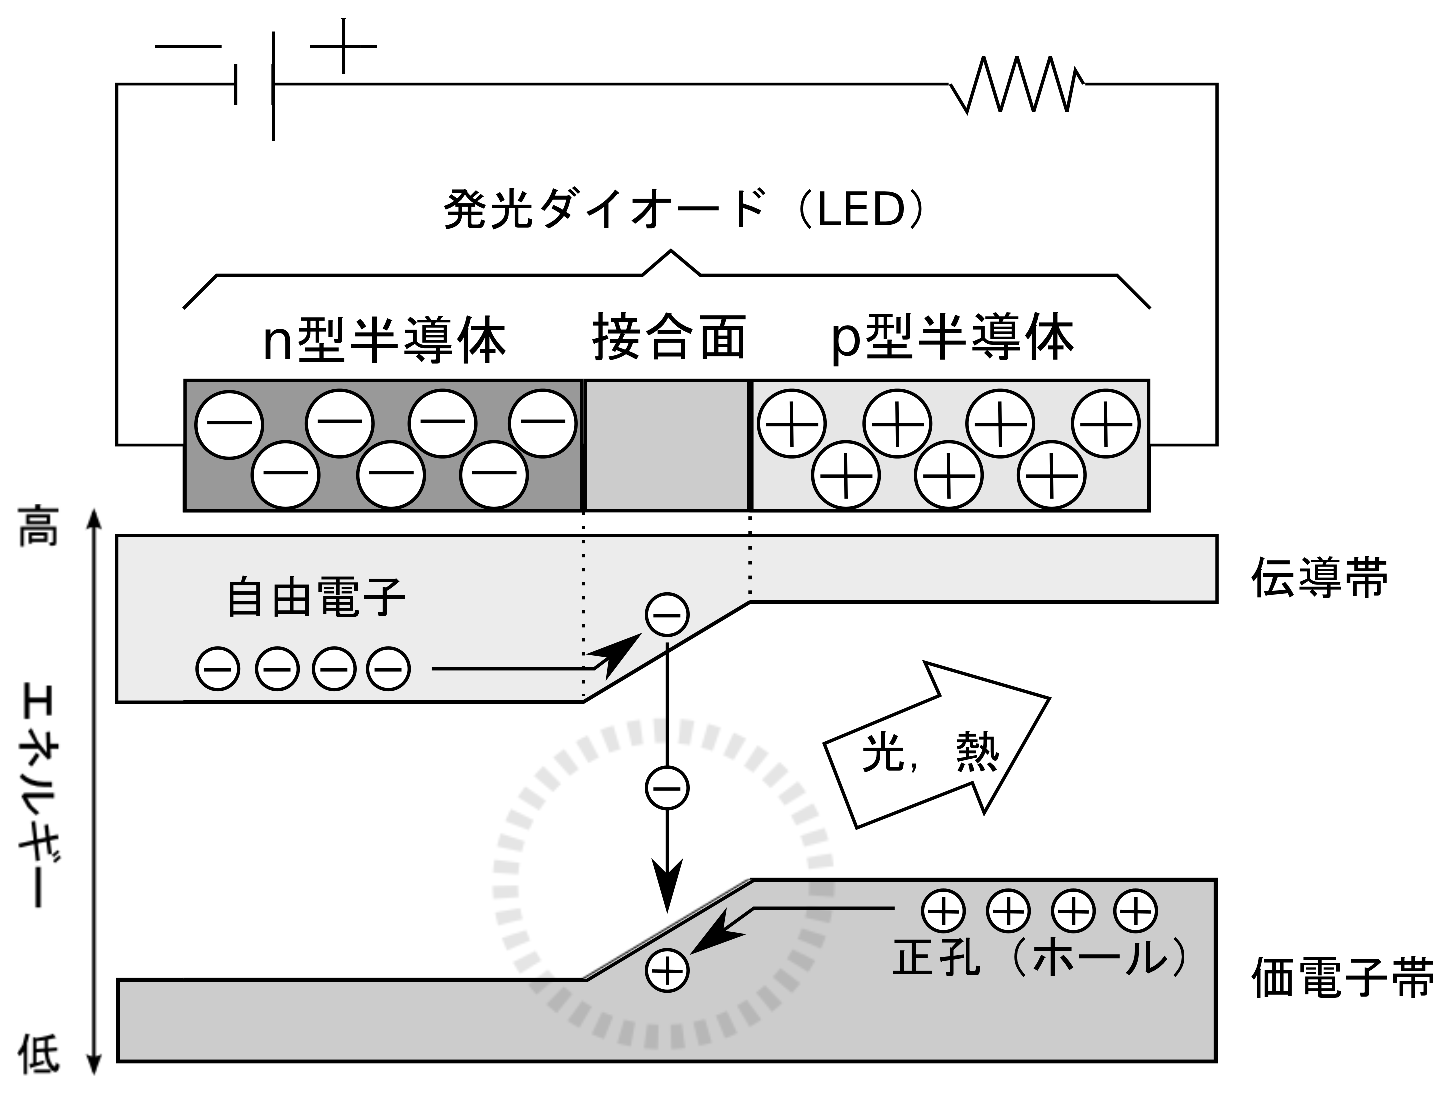
\includegraphics[width=80mm]{img/function.eps}
%\caption{参考画像1}
%\label{led}
%\end{figure}
%
%
%\fgref{sh}を参照します.
%
%\begin{figure}[h]
%
%\centering
%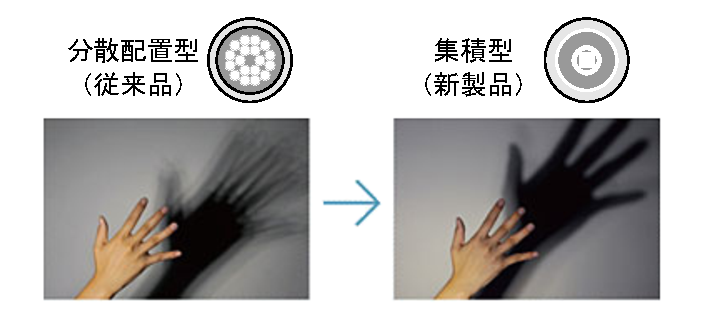
\includegraphics[width=80mm]{img/shade.eps}
%
%縦の空白を挿入する
%\vspace{3cm}
%
%
%\caption{参考画像2}
%\label{sh}
%\end{figure}
%
%
%\section{表を作る}
%
%\begin{table}[h]
%\caption{照明器具の性能比較(参考文献\cite{eru}を参照)}
%\label{table}
%\begin{tabular}{|c|l|l|l|}
%\hline
%  & 白熱電球 & 蛍光灯 & LED照明 \\ \hline
%寿命 & 1000時間 & 10000時間 & 40000時間 \\ \hline
%指向性 & なし & なし & あり\\ \hline
%発光効率 & 10 lm/W & 70 lm/W & 85 lm/W \\
% & & 〜100 lm/W & \\ \hline
%消費電力 & 54 W & 12 W & 7 W\\ \hline
%演色性 & 100 & 84 & 70〜90\\ 
%(Ra) & & & \\ \hline
%発光波長 & 赤外線が & 紫外線が & ほぼ\\
% & 多い & 多い & 可視光線のみ \\ \hline
%電源 & 交流 & 交流 & 直流 \\ \hline
%価格 & - & 白熱電球の & 白熱電球の \\
% & & 20倍 & 80倍 \\ \hline
%\end{tabular}
%\end{table}
%
%縦の空白を挿入する
%
%\tbref{table}を参照します.
%
%
%\vspace{3cm}
%
%\section{箇条書き}
%
%\begin{itemize}
%\item ユニキャスト:他にも
%\item マルチキャスト:「*」などの
%\item エニーキャスト:itemもあります
%\end{itemize}
%
%
%\begin{enumerate}
%\item ユニキャスト:このような
%\item マルチキャスト:番号付き箇条書きも
%\item エニーキャスト:可能です
%\end{enumerate}
%
%\small
%\begin{thebibliography}{99}
%
%\bibitem{SNtech}
%安藤繁,田村陽介,戸辺義人ほか:
%センサネットワーク技術-ユビキタス情報環境の構築に向けて,
%東京電機大学出版局(2005).
%
%\bibitem{reprogramming}
%Wang, Q. and Zhu, Y. and Cheng, L.:
%Reprogramming wireless sensor networks: challenges and approaches,
%{\it Network, IEEE},
%Vol.20,
%No.3,
%pp.48-55(2006).

%% -------------------

%\end{thebibliography}

%% \bibliographystyle{junsrt}
%% \bibliography{bibsample}
\end{document}
